\section{Experiments} \label{sec:experiments}
% \vspace{-8pt}
\subsection{Setup and Data} \label{sec:setup}
The semantic parameters $\mathbf{u}$ we pick are the azimuth rotations of the viewpoint and the elevation angle from the horizontal plane where the object is always at the center of the rendering, which is common in the literature \cite{sada,semantic-attack}. We use 100 shapes from 10 different classes from ShapeNet \cite{shapenet}, the largest dataset for 3D models that are normalized in the semantic lens. We filter these 100 shapes from much more shapes to make sure that: (1) the class label is available in ImageNet and that ImageNet classifiers can identify the exact class, (2) the selected shapes are identified by the classifiers at some part of the semantic space. To do this, we measured the average score in the space and accepted the shape only if its average Resnet softmax score is 0.1. To render the images we use differentiable renderer NMR \cite{vig-nmr} which allows obtaining the gradient to the semantic input parameters.The networks of interest were Resnet50 \cite{resnet}, VGG \cite{vgg}, AlexNet \cite{AlexNet}, and InceptionV3 \cite{inception}. We use the official implementation by Pytorch models \cite{paszke2017pytorch}. this DNNs 
\subsection{Mapping the Networks} \label{sec:maps}
We map the networks similar to \figLabel{\ref{fig:intro_fig}}, but for all the 100 shapes on the first semantic parameter ( the azimuth rotation) as well as the joint (azimuth and elevation) and show the results in \figLabel{\ref{fig:NMS}}. The ranges for the two parameters were [\ang{0},\ang{360}],[\ang{-10},\ang{90}], with 3*3 grid. The total of evaluations is 4K forward passes from every network for every shape ( total of 1.6 M forward passes ). We show all of the remaining results in the \supp ~.

\subsection{Growing Semantic Robust Regions} \label{sec:regions}
We implement the three bottom-up approaches in Table \ref{tbl:complexity} and Algorithms \ref{alg: black} and \ref{alg: white} and open-source the code on GitHub \footnote{https://github.com/ajhamdi/semantic-robustness} and provide a tutorial notebook \footnote{https://colab.research.google.com/drive/1cZzTPu1uwftnRLqtIIjjqw-YZSKh4QYn}. The hyper-parameters were set to $\eta =0.1, \alpha=0.05,  \beta=0.0009 \lambda =0.1, T =800$. We can observe in \figLabel{\ref{fig:operator}} that multiple initial points inside the same robust region converge to the same boundary. One key difference to be noted between the naive approach in \eqLabel{\ref{eq:n-loss-update-naive}} and the OIR formulations in \eqLabel{\ref{eq:n-loss-update-outer},\ref{eq:n-loss-update-grad}} is that naive approach fails to capture robust regions in some scenarios and fall for trivial regions (see \figLabel{\ref{fig:operator}}).
\begin{table}[t]
%\vspace{-8pt}
\small
\tabcolsep=0.09cm
\centering
\begin{tabular}{c|c|cc} 
\toprule
Deep Networ & SRVR & Top-1 error & Top-5 Error \\ 
\midrule
AlexNet \cite{AlexNet} & 8.87\% &43.45   &  20.91 \\
VGG-11 \cite{vgg}& 9.72\%  &30.98  &  11.37   \\
ResNet50 \cite{resnet} &  \textbf{16.79}\% & 23.85      & 7.13  \\
Inceptionv3 \cite{inception}&  7.92\% & \textbf{22.55}  & \textbf{6.44}  \\
\bottomrule
\end{tabular}
\caption{\small \textbf{Benchmarking famous DNNs in Semantic Robustness vs error rate}. We develop Semantic Robustness Volume Ratio (SRVR) metric to estimate semantic robustness of famous Networks in \secLabel{\ref{sec:application}}. We see that semantic robustness doesn't necessarily depends on the accuracy of the DNN, which motivates studying them as an independent metric from the classification accuracy. Errors are reported from Pytorch official implementation, which we use\cite{paszke2017pytorch}.}
% \vspace{-6pt}
\label{tbl:benchmarking}
\end{table}

% width = 2cm
% \begin{figure}[t]
%   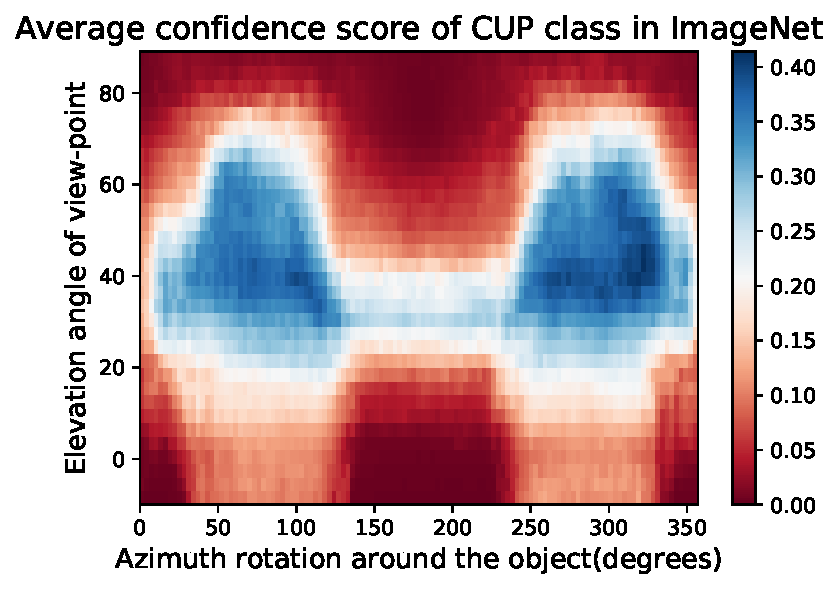
\includegraphics[width=\columnwidth]{images/cup_Average.pdf}
%   \caption{\small \textbf{Semantic Bias in ImageNet}. by taking the verage semantic maps of differnt networks on the CUP class , over 10 shapes, we get a visualization of the bias of the data. Those angles were not probably present in ImageNet\cite{IMAGENET}.}
%   \vspace{-8pt}
%   \label{fig:2d-semantic}
% \end{figure}
% trim={0cm 0cm 0cm 1.1cm},clip, 



\begin{table*}[t]
\footnotesize
\setlength{\tabcolsep}{8pt} % Default value: 6pt
\renewcommand{\arraystretch}{1.1} % Default value: 1
\centering
%\resizebox{0.95\hsize}{!}{
\begin{tabular}{c||c|c|c|c|c|c|c} 
\toprule
\specialcell{\textbf{Analysis}\\ \textbf{Approach}} & \textbf{Paradigm}& \specialcell{\textbf{Total} \\ \textbf{Sampling} \\ \textbf{complexity} } & \specialcell{\textbf{Black} \\\textbf{-box}\\ \textbf{Functions} } & \specialcell{\textbf{Forward} \\ \textbf{pass} \\\textbf{/step} } & \specialcell{\textbf{Backward} \\ \textbf{pass} \\\textbf{/step} } & \specialcell{\textbf{Identification} \\ \textbf{Capabaility} } & \textbf{Hyper-parameters}  \\
\midrule
\textbf{Grid Sampling} &top-down &\specialcell{ $\mathcal{O}(N^{n})$\\$ N \gg 2$  }  & \textcolor{green}{\checkmark} & - & - & \specialcell{Fully identifies the \\semantic map of DNN}  & no hyper-parameters\\ \hline
\textbf{Naive} & bottom-up &$\mathcal{O}(2^{n})$  & \textcolor{green}{\checkmark}& $2^{n}$ &0 & \specialcell{finds strong robust\\ regions only around $\mathbf{u}_{0}$} & \specialcell{$\lambda$, experimentally\\ determined} \\ \hline
\textbf{OIR\_B}& bottom-up &$\mathcal{O}(2^{n+1})$ & \textcolor{green}{\checkmark} & $2^{n+1}$ &0 & \specialcell{finds strong and\\ week robust regions\\ around $\mathbf{u}_{0}$ } & \specialcell{$\alpha$, experimentally\\ determined} \\ \hline
\textbf{OIR\_W}& bottom-up &$\mathcal{O}(2^{n})$ & \textcolor{red}{\xmark}  & $2^{n}$& $2^{n}$ & \specialcell{finds strong and\\ week robust regions\\ around $\mathbf{u}_{0}$ } & \specialcell{$0 \leq \beta < \frac{2}{2n-1}$\\dependeds on $n$ \\ and Lipschitz constant $\mathbb{L}$} \\ 
 \bottomrule
\end{tabular}
%}
\vspace{-4pt}
\caption{\small \textbf{Semantic Analysis Techniques}: comparing different approaches to analyse the semantic robustness of DNN.}
\vspace{-10pt}
\label{tbl:complexity}
\end{table*}
\subsection{Applications} \label{sec:application}

\mysection{Quantifying Semantic Robustness}\\
Looking at these NSM can lead to insights about the network, but we would like to develop a systemic approach to quantify the robustness of these DNNs. To do this, we develop the Semantic Robustness Volume Ratio (SRVR) metric. The SVR metric of the network is only the ratio between the expected size of the robust region obtained by Algorithms \ref{alg: black},\ref{alg: white} over the nominal total volume of the semantic map of interest. Explicitly, the SRVR of network $\mathbf{C}$ for class label z is defined as follows. 

\begin{equation}
\begin{aligned} 
% & \mathbf{\Phi}_{\text{robust}}(f(\mathbf{u}),\mathbf{S}_{z},\mathbf{u}_{0}) = \mathbb{D} = \{\mathbf{u}: \mathbf{a} \leq \mathbf{u} \leq \mathbf{b}\} \\
 \text{SRVR}_{z} =  \frac{\mathbb{E}[\text{Vol}(\mathbb{D})]}{\text{Vol}(\Omega)} = \frac{\mathbb{E}_{\mathbf{u}_{0}\sim \Omega,\mathbf{S}_{z}\sim \mathbb{S}_{z}} [\text{Vol}(\mathbf{\Phi}(f,\mathbf{S}_{z},\mathbf{u}_{0}))]}{\text{Vol}(\Omega)} 
\label{eq:SRVR}
\end{aligned}
\end{equation}
where $f,\Phi$ are defined in \eqLabel{\ref{eq:f},\ref{eq:phi-rob}} respectively. We take the average volume of all the adversarial regions found for multiple initilzations and multiple shapes of the same class $z$ and then divide by the nominal volume of the entire space . This gives a percentage of how close is the DNN from the ideal behaviour of identifying the object robustly in the entire space. The SRVR metric is not strict in its value since the analyzer define the semantic space of interest and the shapes used. However, SRVR relative score from one DNN to another DNN is of extreme importance as it conveys information about the network that might not be clear by only observing the accuracy of the network. For example, we can see in Table \ref{tbl:benchmarking} that while InceptionV3 \cite{inception} is the best in terms of accuracy, it lags behind Resnet50\cite{resnet} in terms of semantic robustness. This observation is also consistent with the qualitative  NSMs in \figLabel{\ref{fig:NMS}} in which we can see that while Inception is very confident, it can fail completely inside these confident regions. Note that the reported SRVR results are averaged over all the 10 classes over all the 100 shapes, and we use 4 constant initial points for all experiments and the semantic parameters are the azimuth and elevation as in \figLabel{\ref{fig:operator},\ref{fig:NMS}}. As can be seen in \figLabel{\ref{fig:operator}} different methods predict different regions , so we take the average size of the the three methods used (naive, OIR\_W, OIR\_B) to give a middle estimate of the volume used in the SRVR results reported in Table \ref{tbl:benchmarking}.


\mysection{Finding Semantic Bias in the Data}\label{sec:data-bias}\\
While looking at the above figures are mesmerizing and can generate a lot of insight about the DNNs and the training data of ImageNet \cite{IMAGENET}, that does not allow to make a conclusion either about the network nor about the data. Therefore, we can average these semantic maps of these networks to factor out the effect of the network structure and training and maintain only the data effect . we show two such maps ( we call Data Semantic Map DSM). We can see that the networks have holes in the semantic maps that are shared among DNNs, indicating bias in the data. Identifying this gap in the data can help training a more semantically robust network by adversarial training on these data-based adversarial regions as performed in the adversarial attack literature \cite{fast-sign}. \figLabel{} shows an example of such semantic map which shows how the data in ImageNet \cite{IMAGENET} did not have such angles of the easy cup class.


\begin{figure}[!t]
    \vspace{-8pt}
  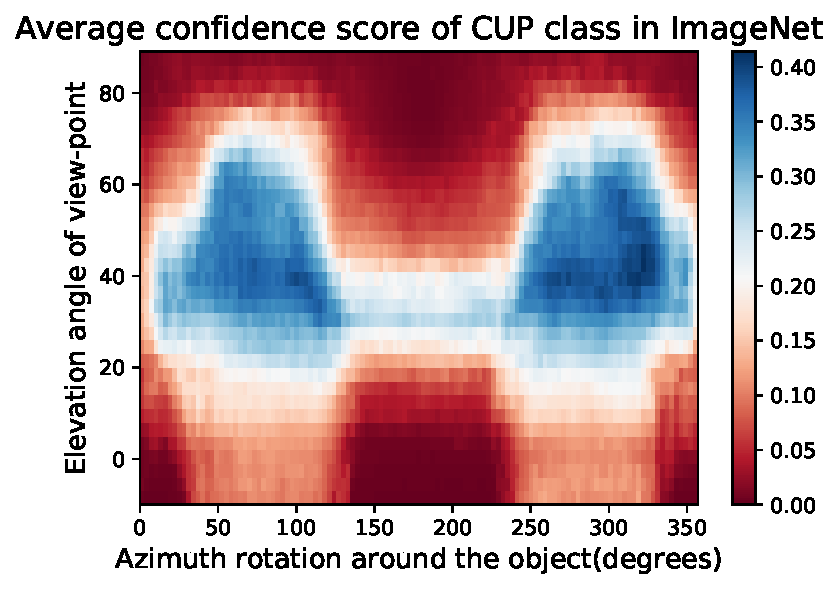
\includegraphics[width=\columnwidth]{images/cup_Average.pdf}
  \vspace{-9pt}
  \caption{\small \textbf{Semantic Bias in ImageNet}. By taking the average semantic maps over 10 shapes of cup class and over different networks, we get a visualization of the bias of the data. Those angles of low score are probably not well-represented in ImageNet\cite{IMAGENET}.}
  \vspace{-10pt}
  \label{fig:2d-semantic}
\end{figure}
